
\documentclass{bredelebeamer}




%%%%%%%%%%%%%%%%%%%%%%%%%%%%%%%%%%%%%%%%%%%%%%%%



\title[Titre version courte]{Ambientes de desenvolvimento para softwares embarcados}
% Titre du diaporama

\subtitle{Buildroot, OpenEmbedded/Yocto}
% Sous-titre optionnel

\author[Oliveira, P. W.]{Phelipe Wesley de Oliveira\inst{1}}
% La commande \inst{...} Permet d'afficher l' affiliation de l'intervenant.
% Si il y a plusieurs intervenants: Marcel Dupont\inst{1}, Roger Durand\inst{2}
% Il suffit alors d'ajouter un autre institut sur le modèle ci-dessous.

\institute[UFC]
{
  \inst{1}%
  Universidade Federal do Ceará
  }


\date{}
% Optionnel. La date, généralement celle du jour de la conférence

\subject{Aula 1}
% C'est utilisé dans les métadonnes du PDF



\logo{

\includegraphics[scale=0.05]{images/logo.png}
}



%%%%%%%%%%%%%%%%%%%%%%%%%%%%%%%%%%%%%%%%%%%%%%%%%%%%%%%%%%%%%%%%%%%%%
\begin{document}

\begin{frame}
  \titlepage
\end{frame}

\logo{}



\begin{frame}{Índice}
  \tableofcontents
  % possibilité d'ajouter l'option [pausesections]
\end{frame}

\section{Introdução}

\begin{frame}{Sistema Embarcado}
	\begin{itemize}
			\item 	Um sistema embarcado, ou sistema embutido, é um sistema 
			microprocessado no qual o computador é completamente encapsulado
			ou dedicado ao dispositivo ou sistema que ele controla.

			\item Um sistema embarcado realiza um conjunto de tarefas 
			pré-definidas, geralmente com requisitos específicos.

			\item Já que o sistema é dedicado à tarefas específicas, 
			pode-se otimizar o sistema reduzindo tamanho, recursos 
			computacionais e custo do produto.
	\end{itemize}
\end{frame}

\begin{frame}
    \frametitle{Sistema Embarcado}
    \begin{itemize}
        \item Costumam fazer uso de microcontroladores.
        \item É necessário programar os microcontroladores.
        \item Existem alguns ambientes de desenvolvimento que facilitam
        essa tarefa.
	\end{itemize}

\end{frame}

\begin{frame}
	\frametitle{MPLAB-X IDE}
	\begin{figure}[htbp]
		\centering
		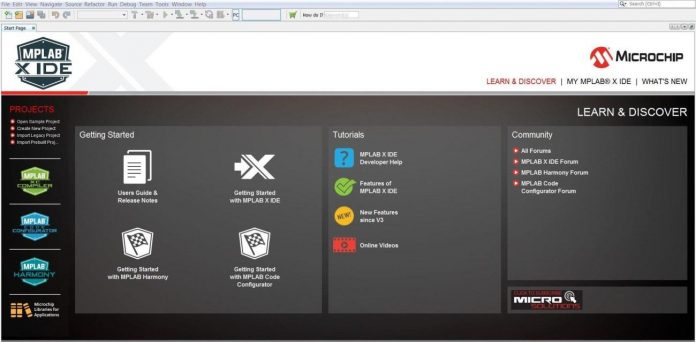
\includegraphics[width=0.9\textwidth]{images/mplab.jpg}
	\end{figure}
\end{frame}

\begin{frame}
	\frametitle{CCS IDE}
	\begin{figure}[htbp]
		\centering
		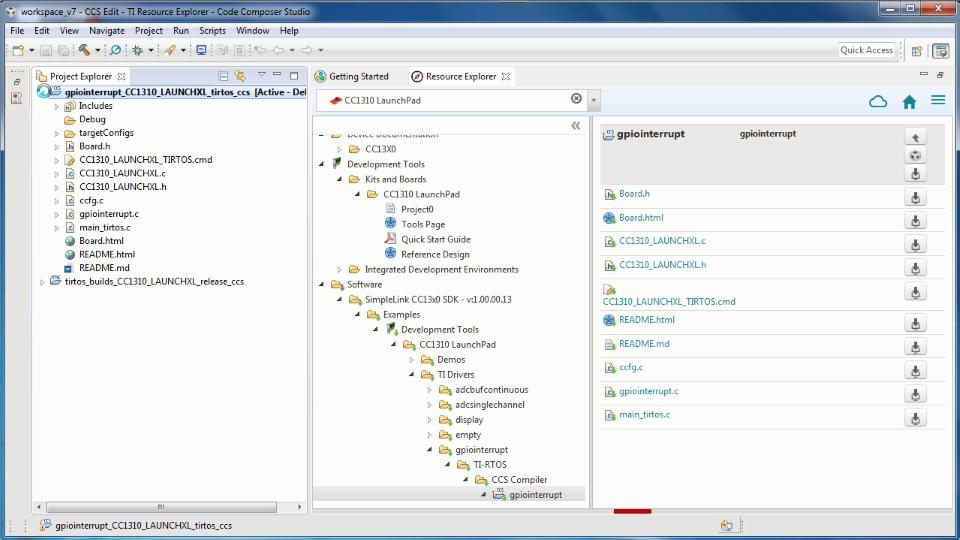
\includegraphics[width=0.9\textwidth]{images/ccs}
	\end{figure}
\end{frame}

\begin{frame}
	\frametitle{Arduino IDE}
	\begin{figure}[htbp]
		\centering
		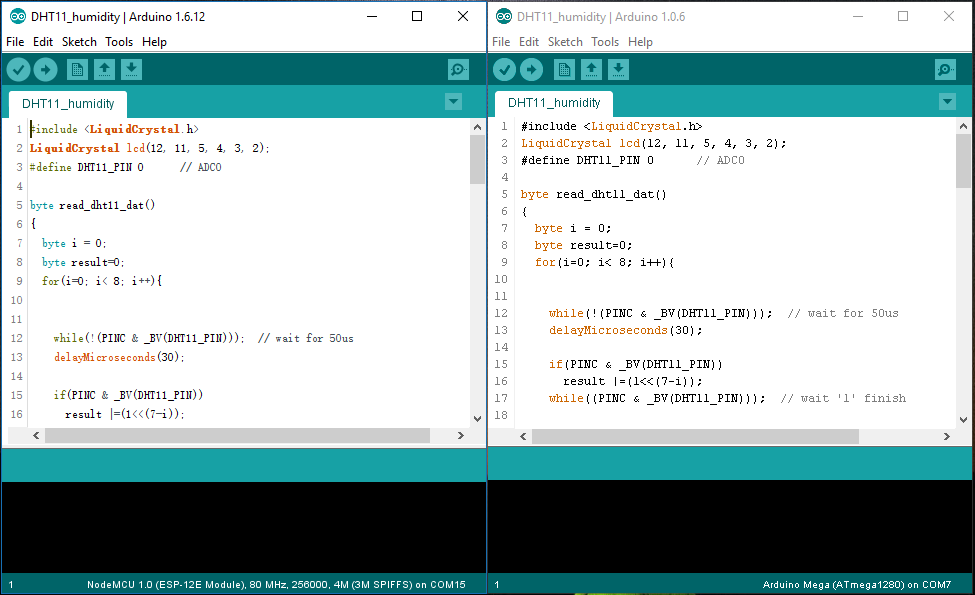
\includegraphics[width=0.8\textwidth]{images/arduino}
	\end{figure}
\end{frame}

\begin{frame}
	\frametitle{Platformio IDE}
	\begin{figure}[htbp]
		\centering
		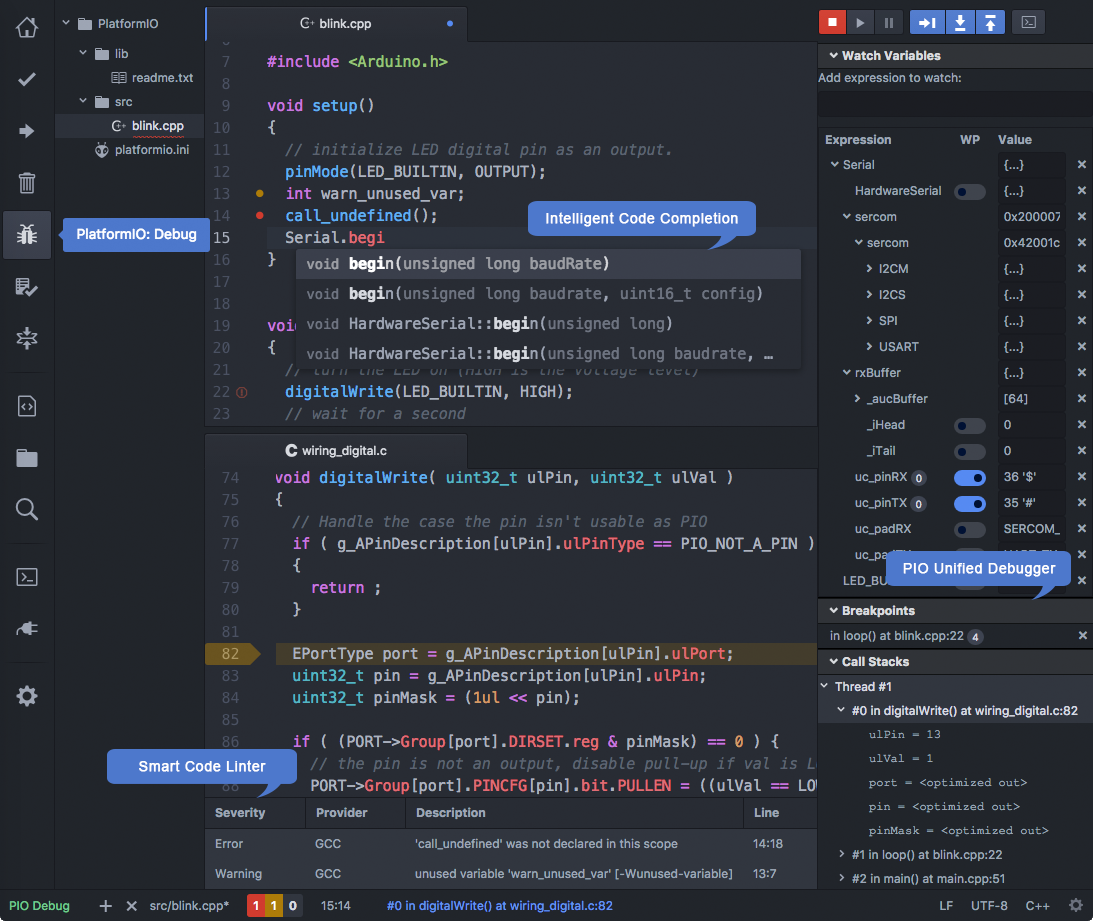
\includegraphics[width=0.8\textwidth]{images/platformio}
	\end{figure}
\end{frame}


\section{Linux Embarcado}

\begin{frame}
    \frametitle{Linux Embarcado}
    \begin{itemize}
        \item Existem aplicações onde somente o uso do 
        microprocessador não é suficiente.
        \item Certas aplicações necessitam de um sistema
        operacional.
        \item O uso de um sistema operacional igual ao dos
        computadores domésticos é inviável pelo excesso de 
        pacotes e funcionalidades desnecessárias.
    \end{itemize}
    

\end{frame}

\begin{frame}
    \frametitle{Linux Embarcado}
    \begin{itemize}
        \item É Necessário criar um sistema operacional customizado
        para o hardware utilizado.
        \item O Linux é comumente utilizado nessas atividades. 
    \end{itemize}
\end{frame}

\begin{frame}
    \frametitle{Linux Embarcado}
    \begin{block}{Linux Embarcado}
        Um sistema Linux Embarcado não se difere conceitualmente 
        de um sistema Linux usado em computadores desktop. A principal
        diferença está na customização e adaptações necessárias para 
        que o Linux seja adaptado ao hardware específico e satisfaça
        os requisitos desejado.
            
    \end{block}    
\end{frame}

\begin{frame}
    \frametitle{Linux Embarcado}
    \begin{figure}[htbp]
        \centering
        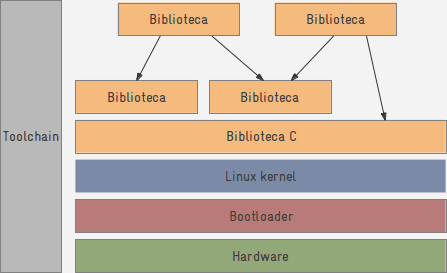
\includegraphics[width=0.9\textwidth]{images/linux-embarcado.png}        
    \end{figure}
    

\end{frame}

\begin{frame}
    \frametitle{Linux Embarcado}
    \begin{enumerate}
        \item    Hardware: o seu produto;
        \item Bootloader: iniciado pelo hardware, responsável pela inicialização 
        básica, carregamento e execução do kernel Linux;
        \item Kernel Linux: núcleo do sistema operacional. Gerencia CPU, memória
        e I/O, exportando serviços para as aplicações do usuário;
        \item Rootfs: sistema de arquivos principal. Possui as bibliotecas do 
        sistema para uso dos serviços exportados pelo kernel, além das 
        bibliotecas e aplicações do usuário;
        \item Toolchain: conjunto de ferramentas para gerar os artefatos de software
        do sistema.
    
    \end{enumerate}
\end{frame}

\begin{frame}
    \frametitle{Linux Embarcado}
    Basicamente, para um sistema Linux Embarcado desempenhar suas funções
    temos que agregar seus diversos artefatos de software - Bootloader,
    Linux Kernel, Bibliotecas, Serviços e Aplicações - para serem executados
    no Hardware alvo. 
    

\end{frame}




\end{document}
